\chapter{Lower bounds for depth-4 circuits with bounded bottom fan-in}

This chapter shall address a recent technique for proving lower bounds for some depth-$4$ circuits. 

\begin{definition}
  A \emph{depth-$4$ circuit}, also referred to as a $\SPSP$ circuit, computes a polynomial of the form 
  $$
  f \spaced{=} Q_{11}\dots Q_{1d} \spaced{+\;\cdots\;+}  Q_{s1}\dots Q_{sd}.
  $$
  The number of summands $s$ is called the \emph{top fan-in} of the circuit. 

  Further, a $\mySPSP{a}{b}$ circuit is a depth-$4$ circuit computing a polynomial of the form
  $$
  f \spaced{=} Q_{11}\dots Q_{1a} \spaced{+\;\cdots\;+}  Q_{s1}\dots Q_{sa}\quad\text{where $\deg Q_{ij} \leq b$ for all $i,j$}.
  $$
\end{definition}

\section{Significance of the model}

In a surprising series of results on depth reduction, Agrawal and Vinay \cite{av08} and subsequent strengthenings of Koiran \cite{koiran} and Tavenas \cite{Tav13} showed that depth-$4$ circuits more or less capture the complexity of general circuits. 

\begin{theorem}[\cite{av08, koiran, Tav13}] 
  If $f$ is an $n$ variate degree-$d$ polynomial computed by a size $s$ arithmetic circuit, then $f$ can also be computed by a $\mySPSP{O(\sqrt{d})}{\sqrt{d}}$ circuit of size $\exp\inparen{O(\sqrt{d}\log s)}$. 
  
  Conversely, if an $n$-variate degree-$d$ polynomial requires $\mySPSP{O(\sqrt{d})}{\sqrt{d}}$  circuits of size $\exp\inparen{\Omega(\sqrt{d}\log s)}$, then it requires arbitrary depth arithmetic circuits of size $n^{\Omega(\log s / \log n)}$ to compute it. 
\end{theorem}

Thus proving strong enough lower bounds for this special case of depth-$4$ circuits imply lower bounds for general circuits. 
The main results of the section is some recent lower bound \cite{gkks13,KSS13,FLMS13} that comes very close to the required threshold. 

\section{Building the complexity measure}

As a simpler task, let us first attempt to prove lower bounds for expressions of the form
$$
f \quad = \quad Q_1^{d} \spaced{+ \;\cdots\; + } Q_s^{d}
$$
where each of the $Q_i$'s are quadratics. 
This is exactly the problem studied by Kayal~\cite{k2}, which led to the complexity measure for proving depth-$4$ lower bounds. \\

The goal is to construct a measure $\Gamma$ such that $\Gamma(f)$ is small whenever $f$ is a power of a quadratic. 
As a first attempt, let us look at the space of $k$-th order partial derivatives of $Q^d$ (for a suitable choice of $k$). 
Unlike the case of $\Sigma\!\wedge\!\Sigma$-circuits where the the space of $k$-th order partial derivatives of $\ell^d$ had dimension $1$, the space of partial derivatives of $Q^{d}$ could be as large as it can be expected. 
Nevertheless, the following simple observation would provide the key intuition.

\begin{observation} 
  Any $k$-th order partial derivative of $Q^d$ is of the form $Q^{d-k}p$ where $p$ is a polynomial of degree at most $k$. 
Hence, if $k \ll d$, then all $k$-th order partial derivatives of $Q^d$ share large common factors.
\end{observation}

This suggests that instead of looking at linear combinations of the partial derivatives of $Q^d$, we should instead be analysing \emph{low-degree polynomial combinations} of them. 
\begin{definition}\label{defn:shifted-partials}
  Let $\partial^{=k}(f)$ refer to the set of all $k$-th order partial derivatives of $f$, and $\vecx^{\leq \ell}$ refer to the set of all monomials of degree at most $\ell$. 
The \emph{shifted partials of $f$}, denoted by $\SPD{k}{\ell}{f}$, is the vector space spanned by $\inbrace{\vecx^{\leq \ell} \cdot \partial^{=k}(f)}$. 
The dimension of this space shall be denoted by $\CM{Kay}_{k,\ell}(f)$. 
\end{definition}

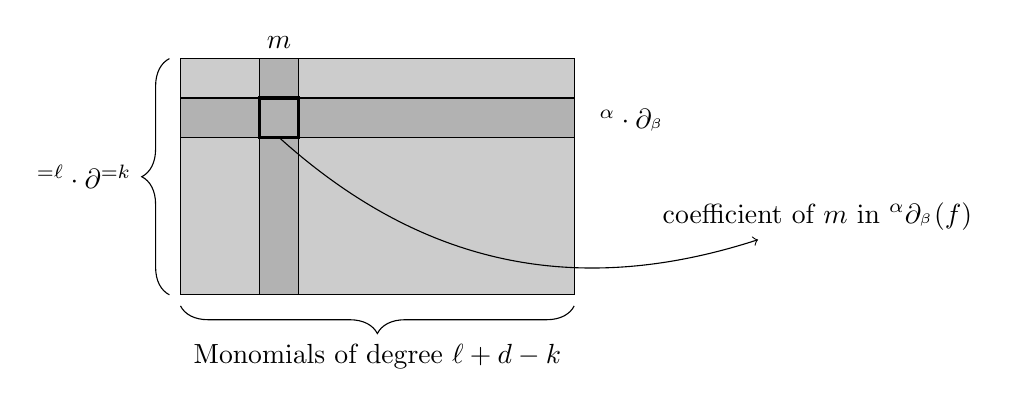
\begin{tikzpicture}
\draw[fill=black!20] (0,0) rectangle (5,3);

\draw[decorate,decoration={brace,amplitude=10pt,raise=4pt},yshift=0pt]
(0,0) -- (0,3);
\node[anchor=east] at (-0.5,1.5) {$\vecx^{=\ell} \cdot \partial^{=k}$};
\draw[decorate,decoration={brace,amplitude=10pt,mirror, raise=4pt},yshift=0pt] 
(0,0) -- (5,0);
\node[anchor=north] at (2.5,-0.5) {Monomials of degree $\ell + d - k$};

\draw[fill=black!30] (1,0) rectangle (1.5,3);
\node at (1.25,3.2) {$m$};

\draw[fill=black!30] (0,2) rectangle (5,2.5);
\node[anchor=west] at (5.2,2.2) {$\vecx^{\alpha} \cdot \partial_{\vecx^\beta}$};

\draw[very thick] (1,2) rectangle (1.5,2.5);

\node[anchor=west] at (6,1) {coefficient of $m$ in $\vecx^\alpha \partial_{\vecx^\beta}(f)$}
edge[<-,bend left] (1.25,2);
\end{tikzpicture}


The above observation shows that any element of $\SPD{k}{\ell}{Q^d}$ is divisible by $Q^{d-k}$ and we thereby have the following lemma. 

\begin{lemma}
  If $f = Q^d$ where $Q$ is a quadratic, then $\CM{Kay}_{k,\ell}(f)\leq \binom{n + k + \ell}{n}$, the number of monomials of degree $(k + \ell)$. 
\end{lemma}

Note that if $f$ was instead a random polynomial, we would expect the measure  $\dim \inparen{\SPD{k}{\ell}{f}}$ to be about $\binom{n+k}{n} \cdot \binom{n+\ell}{n}$, which is \emph{much} larger than $\binom{n+k+\ell}{n}$ for suitable choice of $k,\ell$. 
Hence this measure $\CM{Kay}_{k,\ell}$ is certainly potentially useful for this model. 
Very similar to the above lemma, one can also show the following upper bound for the \emph{building blocks} of $\mySPSP{a}{b}$ circuits. 

\begin{lemma}
Let $f = Q_1\dots Q_a$ with $\deg Q_i \leq b$ for all $i$. 
Then, 
$$
\CM{Kay}_{k,\ell}(f) \spaced{=} \dim \inparen{\SPD{k}{\ell}{f}} \spaced{\leq} \binom{a}{k}\binom{n + (b-1)k + \ell}{n}.
$$
\end{lemma}

It is easy to check that $\CM{Kay}_{k,\ell}$ is a sub-additive measure, and we immediately have this corollary. 

\begin{corollary}\label{cor:dimSPD-upper-bound}
Let $f$ be an $n$-variate polynomial computed by a $\mySPSP{a}{b}$ circuit of top fan-in $s$. 
Then,
$$
\CM{Kay}_{k,\ell}(f) \spaced{\leq} s\cdot \binom{a}{k}\binom{n + (b-1)k + \ell}{n}.
$$
Or in other words for any choice of $k,\ell$, we have that any $\mySPSP{a}{b}$ circuit computing a polynomial $f$ must have top fan-in $s$ at least
$$\frac{\CM{Kay}_{k,\ell}(f)}{\binom{a}{k}\binom{n+(b-1)k + \ell}{n}}.$$ 
\end{corollary}



\subsection*{Intuition from algebraic geometry}

Another perspective for the shifted partial derivatives comes from algebraic geometry. 
Any zero $a\in \F^n$ of $Q$ is a zero of \emph{multiplicity} $d$ of $Q^d$. 
This implies that the set of common zeroes of all $k$-th order partial derivatives of $Q^d$ (for $k \approx  \sqrt{d}$) is \emph{large}. 
On the other hand if $f$ is a random polynomial, then with high probability there are no roots of large multiplicity. 

In algebraic geometry terminology, the common zeroes of a set of polynomials is called the \emph{variety} of the ideal generated by them. 
Further there is also a well-defined notion of a \emph{dimension of a variety} which measures how large a variety is. 
Let $\F[\vecx]_{\leq r}$ refer to the set of polynomials of degree at most $r$, and let $\gamma_I(r) = \dim \inparen{I \intersection \F[\vecx]_{\leq r}}$. 
Intuitively, if $\gamma_I(r)$ is large, then there are \emph{many constraints} and hence the variety is \emph{small}. 
In other words the growth of $\gamma_I(r)$ is inversely related to the dimension of the variety of $I$, and this is precisely captured by what is known as the \emph{Affine Hilbert function of $I$}. 
More about the precise definitions of the Affine Hilbert function etc. can be found in any standard text in algebraic geometry such as \cite{clo}. \\

In our setting, the ideal we are interested in is $I = \inangle{\partial^{=k}f}$. 
If $f$ is a homogeneous polynomial, then $I \intersection \F[\vecx]_{\leq r} = \SPD{k}{\ell}{f}$ where $\ell = r - (\deg(f) - k)$. 
Hence studying the dimension of shifted partial derivatives is exactly studying $\gamma_I(r)$ which holds all information about the dimension of the variety. 

\section{Lower bounding shifted partials of explicit polynomials}

For a random polynomial $R(\vecx)$, we would expect that
$$
\CM{Kay}_{k,\ell}(R) \spaced{\approx} \min\inbrace{\binom{n + \ell + d -k}{n}, \binom{n+k}{n} \binom{n+\ell}{n}}.
$$
The terms on the RHS correspond to trivial upper bounds, where first term is the total number of monomials of degree $(\ell + d-k)$ and the second term is the total number shifted partials.  

\begin{claim}\label{clm:spd-ratio}
For $k = \epsilon \sqrt{d}$ for a small enough $\epsilon > 0$, and $\ell = \frac{c n\sqrt{d}}{\log n}$ for a large enough constant $c$, we have
$$
\frac{\min\inbrace{\binom{n + \ell + d -k}{n}, \binom{n+k}{n} \binom{n+\ell}{n}}}{\binom{O(\sqrt{d})}{k}\binom{n + (\sqrt{d}-1)k + \ell}{n}} \spaced{=} 2^{\Omega(\sqrt{d}\log n)}.
$$
\end{claim}

The proof of this claim is easily obtained by using standard asymptotic estimates of binomial coefficients. 
Note that using \autoref{cor:dimSPD-upper-bound}, the above claim shows that if we can find an explicit polynomial whose dimension of shifted partials are as large as above, then we would have an $\exp(\Omega(\sqrt{d}\log n))$ lower bound for the top fan-in of $\mySPSP{\sqrt{d}}{\sqrt{d}}$ circuits computing this polynomial.\\


If we have a set of polynomials with distinct leading monomials, then they are clearly linearly independent. 
Hence one way of lower bounding the dimension of a space of polynomials is to find a sufficiently large set of polynomials with distinct monomials in the space. 
The vector space of polynomials we are interested is $\SPD{k}{\ell}{f}$, and if we choose a structured polynomial $f$ we can hope to be able to estimate the number of distinct leading monomials in this vector space. 

\subsection{Shifted partials of the determinant and permanent}

The first lower bound for $\mySPSP{\sqrt{d}}{\sqrt{d}}$ circuits was by Gupta, Kamath, Kayal and Saptharishi \cite{gkks13} for the determinant and the permanent polynomial. 
We shall describe the lower bound for $\Det_n$, although it would carry over immediately to $\Perm_n$ as well. 
As mentioned earlier, we wish to estimate the number of distinct leading monomials in $\SPD{k}{\ell}{\Det_n} = \mathrm{span}\inbrace{\vecx^{\leq \ell}\partial^{=k}\Det_n}$. \cite{gkks13} made a relaxation to merely count the number of distinct leading monomials among the generators $\inbrace{\vecx^{\leq \ell}\partial^{=k}\Det_n}$ instead of their span. \\

The first observation is that any $k$-th order partial derivative of $\Det_n$ is just an $(n-k)\times (n-k)$ minor. 
Let us fix a monomial ordering induced by the lexicographic ordering on the variables:
$$
x_{11} \succ x_{12} \dots \succ x_{1n} \succ x_{21} \succ \dots \succ x_{nn}.
$$
Under this ordering, the leading monomial of any minor is just the product of variables on the main diagonal of the sub-matrix corresponding to the minor, and hence is a term of the form $x_{i_1j_1}\dots x_{i_{(n-k)},j_{(n-k)}}$ where $i_1 < \dots < i_{n-k}$ and $j_1 < \dots < j_{n-k}$; let us call such a sequence of indices as an $(n-k)$-increasing sequences in $[n]\times [n]$. 
Further, for any $(n-k)$-increasing sequence, there is a unique minor $M$ whose leading monomial is precisely the product of the variables indexed by the increasing sequence. 
Therefore, the task of lower bounding distinct leading monomials in $\inbrace{\vecx^{\leq \ell}\partial^{=k}\Det_n}$ reduces to the following combinatorial problem.
\begin{claim} For any $k,\ell > 0$,  we have
$$
\CM{Kay}_{k,\ell}(\Det_n) \spaced{\geq} \#\inbrace{\begin{array}{cc}\text{monomials of degree $(\ell + n -k)$ that}\\\text{contain an $(n-k)$-increasing sequence}\end{array}}.
$$
\end{claim}

We could start with an $(n-k)$-increasing sequence, and multiply by a monomial of degree $\ell$ to obtain a monomial containing an increasing sequence. 
Of course, the issue is that this process is not invertible and hence we might overcount. 
To fix this issue, \cite{gkks13} assign a \emph{canonical increasing sequence} to every monomial that contains an increasing sequence and multiply by monomials of degree $\ell$ that do not change the canonical increasing sequence. 

\begin{definition}
Let $D_2 = \inbrace{x_{1,1},\dots, x_{n,n}, x_{1,2},x_{2,3}, \dots, x_{n-1,n}}$, the main diagonal and the diagonal just above it. 
For any monomial $m$ define the \emph{canonical increasing sequence of $m$}, denoted by $\chi(m)$, as $(n-k)$-increasing sequence of $m$ that is entirely contained in $D_2$ and is ordered highest according to the ordering '$\succ$'. 
If $m$ contains no $(n-k)$-increasing sequence entirely in $D_2$, then we shall say the canonical increasing sequence is empty. 
\end{definition}

The reason we restrict ourselves to $D_2$ is because it is easier to understand which monomials change the canonical increasing sequence and which monomials do not. 

\begin{lemma}\label{lem:forbidden-variables}
Let $S$ be an $(n-k)$-increasing sequence completely contained in $D_2$, and let $m_S$ be the monomial obtained by multiplying the variables indexed by $S$. 
There are at least $(2(n-k)-1)$ variables in $D_2$ such that if $m$ is any monomial over these variables, then $\chi(m_S) = \chi(m\cdot m_S)$. 
\end{lemma}
\begin{proof}
Note that for any $x_{i,j} \in D_2$ other than $x_{n,n}$, exactly one of $x_{i+1,j}$ or $x_{i,j+1}$ is in $D_2$ as well; let us refer to this element in $D_2$ as the \emph{companion} of $x_{i,j}$. 
It is straightforward to check that for any $(n-k)$-increasing sequence $S$, the elements of $S$ and their companions do not alter the canonical increasing sequence. 
\end{proof}

It is a simple exercise to check that the number of $(n-k)$-increasing sequences contained in $D_2$ is $\binom{n+k}{2k}$. 
Further, as we are free to use the $n^2 - 2n + 1$ variables outside $D_2$, and the $2(n-k) -1$ variables that don't alter the canonical increasing sequence, we have the following lemma. 

\begin{lemma}\label{lem:dimSPD-det-lb}
For any $k,\ell \geq 0$, 
$$
\dim\inparen{\SPD{k}{\ell}{\Det_n}} \spaced{\geq} \binom{n+k}{2k}\binom{(n^2 - 2n + 1) + 2(n-k) -1 + \ell}{\ell}.
$$
\end{lemma}

Although this lower bound is not as large as expected for a random polynomial, this is still sufficient to give strong lower bounds for depth-$4$ circuits. 
By choosing $k = \epsilon \sqrt{n}$ for a small enough $\epsilon > 0$, and $\ell = n^2 \sqrt{n}$, \autoref{lem:dimSPD-det-lb} with \autoref{cor:dimSPD-upper-bound} yields the lower bound of Gupta, Kamath, Kayal and Saptharishi \cite{gkks13}

\begin{theorem}
Any $\mySPSP{O(\sqrt{n})}{\sqrt{n}}$ circuit computing $\Det_n$ or $\Perm_n$ has top fanin $2^{\Omega(\sqrt{n})}$. \qed
\end{theorem}

It is worth noting that although \autoref{clm:spd-ratio} suggests that we should be able to obtain a lower bound of $\exp(\Omega(\sqrt{n}\log n))$ for $\Det_n$, \cite{gkks13} also showed that the above estimate for the dimension of shifted partial derivatives for the determinant is fairly tight. 
Hence the dimension of shifted partials cannot give a stronger lower bound for the determinant polynomial. 
However, it is possible that the estimate is \emph{not} tight for the permanent and the dimension of shifted partial derivatives of the permanent is provably strictly larger than that of the determinant! 
It is conceivable that one should be able to prove an $\exp(\Omega(\sqrt{n}\log n))$ lower bound for the permanent using this measure. 

Indeed, subsequently an $\exp(\Omega(\sqrt{d}\log n))$ was proved \cite{KSS13,FLMS13} for other explicit polynomials  which we now outline. 

\subsection{Shifted partials of the Nisan-Wigderson polynomial}

Very shortly after \cite{gkks13}'s $2^{\Omega(\sqrt{n})}$ lower bound, Kayal, Saha and Saptharishi \cite{KSS13} gave a stronger lower bound for a different polynomial. 
Their approach was to engineer an explicit polynomial $F$ for which the dimension of shifted partial derivatives is easier to estimate. 
The main idea was that, if any $k$-th order partial derivative of the engineered polynomial is a monomial, then once again estimating $\dim\inparen{\SPD{k}{\ell}{F}}$ reduces to a monomial counting problem. 
If we could ensure that no two monomials of $F$ have a gcd of degree $k$ or more, then we would immediately get that all $k$-th order partial derivatives of $F$ are just monomials (albeit possibly zero). 
If we were to interpret the set of non-zero monomials of $F$ as just subsets over the variables, then the above constraint can be rephrased as a set system with \emph{small pairwise intersection}. 
Such systems are well studied and are known as Nisan-Wigderson designs \cite{nw94}. 
With this in mind, \cite{KSS13} studied the following polynomial family inspired by an explicit construction of a Nisan-Wigderson design. 
The definition below is a specialization of \autoref{defn:NW-polyfamilies}. 

\begin{definition}[Nisan-Wigderson Polynomial]. 
Let $n$ be a power of $2$ and let $\F_n$ be the finite field with $n$ elements that are identified with the set $\inbrace{1,\dots, n}$. 
For any $0\leq k \leq n$, the polynomial $\mathrm{NW}_k$ is a $n^2$-variate polynomial of degree $n$ defined as follows:
$$
\mathrm{NW}_k(x_{1,1},\dots, x_{n,n}) \spaced{=} \sum_{\substack{p(t) \;\in\; \F_n[t]\\\deg(p) \;<\; k}} x_{1,p(1)}\dots x_{n,p(n)}.
$$
\end{definition}

We recall the main observation about the set of monomials of the Nisan-Wigderson polynomial which is the \emph{low pairwise-intersection} property. 

\begin{observation}
Any two monomials of $\mathrm{NW}_k$ intersect in less than $k$ variables. 
Hence, any $k$-th order partial derivative of $\mathrm{NW}_k(\vecx)$ is a monomial (which could possibly be zero). \qed
\end{observation}

Hence, the problem of lower bounding the shifted partials of $\mathrm{NW}_k$ reduces to the problem of counting distinct monomials of degree $\ell + d-k$ that are divisible by one of these $k$-th order derivatives. \cite{KSS13} additionally used the observation that two random $k$-th order partial derivatives of $\mathrm{NW}_k$ are monomials that are \emph{far} from each other. 
Using this, they estimate the number of distinct shifts of these monomials and showed that the dimension of shifted partial derivatives of $\mathrm{NW}_k$ is very close to the trivial upper bound as in \autoref{clm:spd-ratio}. 
We sketch the argument by Chillara and Mukhopadhyay \cite{cm14}. 
Formally, for any two multilinear monomials $m_1$ and $m_2$, let the $\Delta(m_1,m_2)$ denote $\min\inbrace{|m_1| - |m_1\intersection m_2|, m_2 - |m_1 \intersection m_2|}$ (abusing notation by identifying the multilinear monomials with the set of variables that divide it). 

\begin{lemma}[\cite{cm14}]\label{lem:cm-inc-exc}
Let $m_1,\dots, m_s$ be monomials over $N$ variables such that $\Delta(m_i, m_j) \geq d$ for all $i\neq j$. 
Then the number of distinct monomials that may be obtained by multiplying some $m_i$ by arbitrary monomials of degree $\ell$ is at least $s \binom{N+\ell}{N} - \binom{s}{2} \binom{N+\ell - d}{N}$. 
\end{lemma}
\begin{proof}
For $i = 1,\dots, s$, let $A_i$ be the set of monomials that can be obtained by multiplying $m_i$ with a degree $\ell$ monomial. 
By inclusion-exclusion, 
$$
\abs{\Union_{i=1}^s A_i} \spaced{\geq} \sum_{i=1}^s \abs{A_i} \spaced{-} \sum_{i<j} \abs{A_i \intersection A_j}.
$$
Note that each $A_i$ is of size exactly $\binom{N+\ell}{N}$. 
Further, since $\Delta(m_i, m_j) \geq d$, any monomial that is divisible by $m_i$ and $m_j$ must necessarily be divisible by $m_i$ and the variables in $m_j$ not in $m_i$. 
Hence, $\abs{A_i\intersection A_j} \leq \binom{N + \ell - d}{N}$. 
The lemma follows by substituting these above. 
\end{proof}

Note that any two distinct monomials of $\mathrm{NW}_k$ intersect in at most $k$ places. 
For each monomial $m_i$ of $\mathrm{NW}_k$, let $m_i'$ be any non-zero $k$-th order partial derivative of $m_i$. 
Therefore, $\Delta(m_i', m_j') \geq n -2k \geq \frac{n}{2}$ for $k = \epsilon \sqrt{n}$. 
Since we have $n^k$ monomials of pairwise distance at least $n/2$, the above lemma immediately yields a lower bound for the shifted partials of $\mathrm{NW}_k$. 

\begin{theorem}[\cite{KSS13}]
Let $k = \epsilon \sqrt{d}$ for some constant $\epsilon > 0$. 
Then for any  $\ell = \Theta\inparen{\frac{n^2 \sqrt{n}}{\log n}}$,
$$
\dim\inparen{\SPD{k}{\ell}{\mathrm{NW}_k}} \spaced{\geq} \frac{n^k}{2} \cdot \binom{n^2 + \ell}{n^2}
$$
\end{theorem}
\begin{proof-sketch}
As mentioned earlier, we have $n^k$ monomials $\inbrace{m_i'}$ with pairwise distance at least $\frac{n}{2}$. 
Using \autoref{lem:cm-inc-exc}, it suffices to show that
$$
n^k \cdot \binom{n^2 + \ell}{n^2} \spaced{\geq} 2 \cdot \binom{n^k}{2} \cdot \binom{n^2 + \ell - \frac{n}{2}}{n^2}
$$
and this follows easily from standard binomial coefficient estimates. 
\end{proof-sketch}

Combining with \autoref{cor:dimSPD-upper-bound}, we have the lower bound of \cite{KSS13} using standard estimates. 

\begin{theorem}[\cite{KSS13}]
Any $\mySPSP{O(\sqrt{n})}{\sqrt{n}}$ computing the $\mathrm{NW}_k$ polynomial, where $k = \epsilon \sqrt{n}$ for a sufficiently small $\epsilon > 0$, must have top fan-in $\exp(\Omega(\sqrt{n}\log n))$. \qed
\end{theorem}

\cite{KSS13} used the above lower bound to give an $n^{\Omega(\log n)}$ lower bound for a subclass of formulas called \emph{regular formulas}. 
The interested reader can refer to \cite{KSS13} for more details. 

\subsection{Shifted partials of the Iterated-matrix-multiplication polynomial}

Fourier, Limaye, Malod and Srinivasan \cite{FLMS13} showed the same lower bound as \cite{KSS13} but for the \emph{iterated matrix multiplication} polynomial which is known to have polynomial sized circuits computing it. 

\begin{definition}[Iterated matrix multiplication polynomial]
Let $M_1,\dots, M_d$ be $n\times n$ matrices with distinct variables as entries, i.e. $M_k = \inparen{\!\!\inparen{x_{ij}^{(k)}}\!\!}_{i,j\leq n}$ for $k = 1,\dots, d$. 
The polynomial $\mathrm{IMM}_{n,d}$ is a $(n^2d)$-variate degree-$d$ polynomial defined as the $(1,1)$-th entry of the matrix product $M_1\dots M_d$:
$$
\mathrm{IMM}_{n,d}(\vecx) \spaced{=} \inparen{M_1 \dots M_d}_{1,1}.
$$
\end{definition}

A more useful perspective is to interpret this as a \emph{canonical algebraic branching program}. 

\begin{definition}[Algebraic branching program]
An algebraic branching program (ABP) comprises of a layered directed graph $G$ with $(d+1)$ layers of vertices, where the first and last layer consists of a single node (called source and sink respectively), all other layers consist of $n$ vertices, and edges are only between successive layers and have linear polynomials as edge-weights. 
The ABP is set to compute the polynomial $f$ defined as
$$
f(\vecx) \spaced{=} \sum_{\text{source-sink path $\rho$}} \mathrm{weight}(\rho)
$$
where the $\mathrm{weight}$ of any path is just the product of the edge weights on the path. 
\end{definition}

The canonical ABP comprises of the graph where the $i$-th vertex of layer $(\ell-1)$ is connected to the $j$-th vertex of layer $\ell$ with edge-weight $x_{ij}^{(\ell)}$ for every choice of $i,j$ and $\ell$. 
It is easy to see that the polynomial computed by the canonical ABP is in fact $\mathrm{IMM}_{n,d}$. \\

To lower bound the dimension of shifted partial derivatives of $\mathrm{IMM}_{n,d}$, firstly note that a derivative with respect to any variable (or edge) simply results in the sum of all source-sink paths that \emph{pass} through this edge. \cite{FLMS13} use the following simple but crucial observation to assist in bounding the dimension of shifted partials. 

\begin{observation}\label{obs:odd-layer-unique-path}
Assume that $d$ is even. 
Let $e_1,e_3,\dots, e_{d-1}$ be an arbitrary set of edges such that $e_i$ is between layer $i$ and $i+1$. 
Then, there is a unique path from source to sink that passes through all these edges. 
\end{observation}
\begin{proof}
Since these are edges in alternate layers, their starting and ending points uniquely determine the edges that are picked up from the even-numbered layers to complete the source-sink path.
\end{proof}

Since we are interested in $k$-th order derivatives for $k \approx \epsilon \sqrt{d}$, \cite{FLMS13} consider the following restriction by removing some edges from the underlying graph:
\begin{itemize}
\item Select $(2k-1)$ layers $\ell_1,\dots, \ell_{2k-1}$ that are roughly equally spaced between the first and the last layer. 
These layers, and the first and the last layers, shall be untouched and shall be called \emph{pristine layers}.
\item In all the other layers, retain only those edges connecting vertex $i$ of this layer to vertex $i$  of the next. 
\end{itemize}
This restriction effectively makes the graph similar to an ABP with $2k+1$ layers. 
Let the polynomial computed by the restricted ABP be $\mathrm{IMM}'_{n,d}(\vecx)$. 
Since $\mathrm{IMM}'_{n,d}$ was obtained by just setting some variables of $\mathrm{IMM}_{n,d}$ to zero, the dimension of shifted partial derivatives of $\mathrm{IMM}'_{n,d}$ can only be smaller than that of $\mathrm{IMM}_{n,d}$. 
Similar to \autoref{obs:odd-layer-unique-path}, we have the following observation. 

\begin{observation}
For every choice of $k$ edges from odd-numbered pristine layers, there is a unique source-sink path that passes through them. 

In other words, for any choice of $k$ variables chosen by picking one from each odd-numbered pristine layer, then the $k$-th order partial derivative of $\mathrm{IMM}'_{n,d}$ with respect to these $k$ variables is a non-zero monomial. 
\end{observation}

Once again, we can lower bound the dimension of shifted partial derivatives of $\mathrm{IMM}'_{n,d}$ by a monomial counting problem. 
Similar to the earlier case, \cite{FLMS13} show that the monomials thus obtained are \emph{far} from one another. 
We state their main lemma below without proof. 

\begin{lemma}[\cite{FLMS13}]
There are at least $n^{k/2}$ monomials of $\mathrm{IMM}'_{n,d}$ of pairwise distance at least $\frac{n}{4}$. 
\end{lemma}

Again, using \autoref{lem:cm-inc-exc} and standard binomial coefficient estimates, this implies that the shifted partial derivatives of $\mathrm{IMM}'_{n,d}$ is almost as large as the trivial upper bound. 

\begin{theorem}[\cite{FLMS13}]Let $k = \epsilon\sqrt{d}$ for a sufficiently small $\epsilon > 0$ and $\ell$ be an integer such that $n^{1/16} \leq \frac{N + \ell}{\ell} \leq n^{1/4}$ where $N$ is the number of variables $\mathrm{IMM}_{n,d}'$ depends on. 
Then, 
\begin{eqnarray*}
\dim\inparen{\SPD{k}{\ell}{\mathrm{IMM}_{n,d}}} &\geq& \dim\inparen{\SPD{k}{\ell}{\mathrm{IMM}'_{n,d}}} \\
& =& \Omega\inparen{n^{k/2} \cdot \binom{N + \ell}{\ell}}.
\end{eqnarray*}
\qed
\end{theorem}

Combining with \autoref{cor:dimSPD-upper-bound}, we get the lower bound of \cite{FLMS13}. 

\begin{theorem}[\cite{FLMS13}]
Any $\mySPSP{O(\sqrt{d})}{\sqrt{d}}$ circuit computing $\mathrm{IMM}_{n,d}$, with $d \leq n^{\delta}$ for a sufficiently small $\delta > 0$, has top fan-in $\exp(\Omega(\sqrt{d}\log n))$. \qed
\end{theorem}

Similar to \cite{KSS13}, the above result also implies $n^{\Omega(\log n)}$ lower bounds for regular formulas computing $\mathrm{IMM}_{n,d}$. 


%%% Local Variables: 
%%% mode: latex
%%% TeX-master: "main"
%%% End: 

